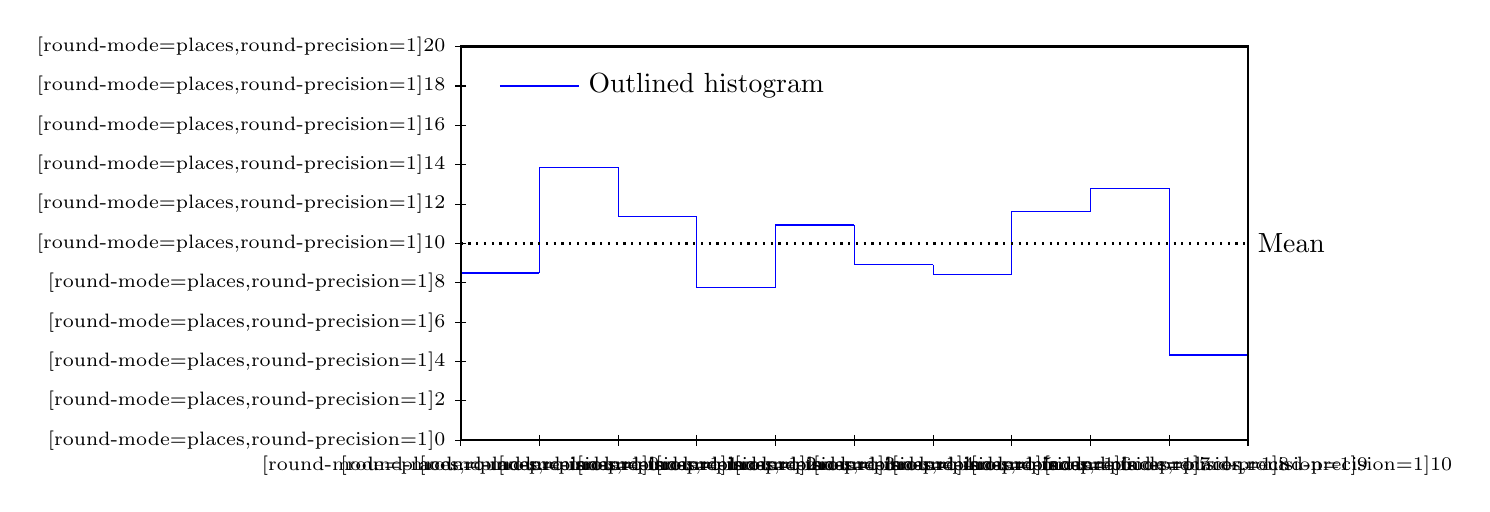
\begin{tikzpicture}
\begin{scope}
\clip (0,0) rectangle (10,5);
\draw[blue] (0.0,2.1250264973793005) -- (1.0,2.1250264973793005);
\draw[blue] (1.0,2.1250264973793005) -- (1.0,3.4654917134985634) -- (2.0,3.4654917134985634);
\draw[blue] (2.0,3.4654917134985634) -- (2.0,2.8394039376901827) -- (3.0,2.8394039376901827);
\draw[blue] (3.0,2.8394039376901827) -- (3.0,1.935008777053877) -- (4.0,1.935008777053877);
\draw[blue] (4.0,1.935008777053877) -- (4.0,2.7339057883083795) -- (5.0,2.7339057883083795);
\draw[blue] (5.0,2.7339057883083795) -- (5.0,2.229137762837512) -- (6.0,2.229137762837512);
\draw[blue] (6.0,2.229137762837512) -- (6.0,2.107856772034629) -- (7.0,2.107856772034629);
\draw[blue] (7.0,2.107856772034629) -- (7.0,2.9034298388534907) -- (8.0,2.9034298388534907);
\draw[blue] (8.0,2.9034298388534907) -- (8.0,3.2007256875659142) -- (9.0,3.2007256875659142);
\draw[blue] (9.0,3.2007256875659142) -- (9.0,1.0831759093161741) -- (10.0,1.0831759093161741);
\end{scope}
\draw (0,0cm + 2pt) -- (0, 0cm -2pt) node[below] {\scriptsize{\num[round-mode=places,round-precision=1]{0}}};
\draw (1,0cm + 2pt) -- (1, 0cm -2pt) node[below] {\scriptsize{\num[round-mode=places,round-precision=1]{1}}};
\draw (2,0cm + 2pt) -- (2, 0cm -2pt) node[below] {\scriptsize{\num[round-mode=places,round-precision=1]{2}}};
\draw (3,0cm + 2pt) -- (3, 0cm -2pt) node[below] {\scriptsize{\num[round-mode=places,round-precision=1]{3}}};
\draw (4,0cm + 2pt) -- (4, 0cm -2pt) node[below] {\scriptsize{\num[round-mode=places,round-precision=1]{4}}};
\draw (5,0cm + 2pt) -- (5, 0cm -2pt) node[below] {\scriptsize{\num[round-mode=places,round-precision=1]{5}}};
\draw (6,0cm + 2pt) -- (6, 0cm -2pt) node[below] {\scriptsize{\num[round-mode=places,round-precision=1]{6}}};
\draw (7,0cm + 2pt) -- (7, 0cm -2pt) node[below] {\scriptsize{\num[round-mode=places,round-precision=1]{7}}};
\draw (8,0cm + 2pt) -- (8, 0cm -2pt) node[below] {\scriptsize{\num[round-mode=places,round-precision=1]{8}}};
\draw (9,0cm + 2pt) -- (9, 0cm -2pt) node[below] {\scriptsize{\num[round-mode=places,round-precision=1]{9}}};
\draw (10,0cm + 2pt) -- (10, 0cm -2pt) node[below] {\scriptsize{\num[round-mode=places,round-precision=1]{10}}};
\draw (0cm + 2pt,0.    ) -- (0cm-2pt,0.    ) node[left] {\scriptsize{\num[round-mode=places,round-precision=1]{0}}};
\draw (0cm + 2pt,0.5    ) -- (0cm-2pt,0.5    ) node[left] {\scriptsize{\num[round-mode=places,round-precision=1]{2}}};
\draw (0cm + 2pt,1.    ) -- (0cm-2pt,1.    ) node[left] {\scriptsize{\num[round-mode=places,round-precision=1]{4}}};
\draw (0cm + 2pt,1.5    ) -- (0cm-2pt,1.5    ) node[left] {\scriptsize{\num[round-mode=places,round-precision=1]{6}}};
\draw (0cm + 2pt,2.    ) -- (0cm-2pt,2.    ) node[left] {\scriptsize{\num[round-mode=places,round-precision=1]{8}}};
\draw (0cm + 2pt,2.5    ) -- (0cm-2pt,2.5    ) node[left] {\scriptsize{\num[round-mode=places,round-precision=1]{10}}};
\draw (0cm + 2pt,3.    ) -- (0cm-2pt,3.    ) node[left] {\scriptsize{\num[round-mode=places,round-precision=1]{12}}};
\draw (0cm + 2pt,3.5    ) -- (0cm-2pt,3.5    ) node[left] {\scriptsize{\num[round-mode=places,round-precision=1]{14}}};
\draw (0cm + 2pt,4.    ) -- (0cm-2pt,4.    ) node[left] {\scriptsize{\num[round-mode=places,round-precision=1]{16}}};
\draw (0cm + 2pt,4.5    ) -- (0cm-2pt,4.5    ) node[left] {\scriptsize{\num[round-mode=places,round-precision=1]{18}}};
\draw (0cm + 2pt,5.    ) -- (0cm-2pt,5.    ) node[left] {\scriptsize{\num[round-mode=places,round-precision=1]{20}}};
\draw[thick] (0,0) rectangle (10,5);
\draw[thick,dotted] (0.0,2.5) -- (10.0,2.5);
\node[right] at (10.0,2.5) {Mean};
\draw[blue] (0.5,4.5) -- (1.5,4.5);
\node[right,] at (1.5,4.5) {Outlined histogram};
\end{tikzpicture}
%%% Local Variables: 
%%% mode: latex 
%%% TeX-master: "master" 
%%% End:

